\documentclass[a4paper, fontsize=14pt]{article}
\usepackage{scrextend}
\usepackage{indentfirst, fancyhdr, amsfonts, mathtools, amssymb}
\usepackage{titlesec} %работа с рубрикацией
\usepackage{tocloft} %настройки оглавления
\usepackage[T2A]{fontenc}
\usepackage[utf8x]{inputenc}
\usepackage[russian]{babel}
\usepackage{hyperref} %кликабельное оглавление
\usepackage[left=3.7cm,right=2cm,top=2cm,bottom=2cm]{geometry}
\usepackage{tempora} %настраиваем шрифт типа TNR                                   
\usepackage{newtxmath} %делаем шрифт формул похожим на TNR
\usepackage[labelsep=endash]{caption}
\usepackage{listings}
\usepackage{ucs}
\usepackage{amsmath}
\usepackage{pdfpages}
\usepackage{tocloft}
\usepackage{textcase}
\usepackage{textcomp}
\renewcommand\cftsecafterpnum{\vskip15pt}
\lstset{
  columns=fullflexible,
  breaklines=true,
}
\linespread{1}
\setcounter{page}{1} %в зависимости от того, какой по счёту страницей должно быть оглавление!

%НАСТРОЙКИ ОГЛАВЛЕНИЯ

\renewcommand{\cftsecaftersnum}{.} %точки после номеров разделов и подразделов в оглавлении
\renewcommand{\cftsubsecaftersnum}{.}
\renewcommand{\cftsecfont}{\normalfont} %разделы в оглавлении пишутся обычным (не жирным) шрифтом
\renewcommand{\cftsecpagefont}{\normalfont} %соответствующие им страницы тоже
\renewcommand{\cftsecleader}{\cftdotfill{\cftdotsep}} %расставляем точки между названиями разделов и их страницами
\addto\captionsrussian{\renewcommand\contentsname{СОДЕРЖАНИЕ}} %хотим, чтобы слово "Содержание" писалось капсом
\renewcommand{\cfttoctitlefont}{\hfil\bfseries} %слово СОДЕРЖАНИЕ по центру жирным
\renewcommand{\cftaftertoctitle}{\hfill}
% \renewcommand{\cftsecfont}{\MakeUppercase}

\captionsetup[figure]{name=Рисунок}
%НАСТРОЙКИ РУБРИКАЦИИ
\titleformat*{\section}{\center\bf} %названия разделов и подразделов по середине жирным шрифтом
\titleformat*{\subsection}{\center\bf}
\titlelabel{\thetitle.\quad} %название раздела и его номер отделены точкой

%НАСТРОЙКИ БИБЛИОГРАФИИ
\addto\captionsrussian{\renewcommand\refname{СПИСОК ЛИТЕРАТУРЫ}} %хотим, чтобы слова "Список литературы" писались капсом
\makeatletter
\renewcommand{\@biblabel}[1]{#1.} %хотим, чтобы в списке литературы номера источников писались в формате "No. <...>", а не "[No] <...>"
\makeatother
\newtheorem{definition}{Определение}

% НАСТРОЙКИ ПРОИЗВОДНЫХ
\newcommand{\MD}[2]{\mathbb{D}_{#1}^{\alpha}[#2]} % Marchaud derivative
\newcommand{\RLD}[3]{{}_{#1}\mathcal{D}_{#2}^{\alpha} \left[#3\right]} % Riemann Liuville derivative
\newcommand{\D}[3]{D_{#1}^{#2} \left[ #3 \right]} % Riemann Liuville derivative

\newcommand{\RLDa}[4]{{}_{#1}\mathcal{D}_{#2}^{#4} \left[#3\right]} % Riemann Liuville derivative with var alpha

\newcommand{\RLI}[3]{{}_{#1}\mathcal{I}_{#2}^{\alpha} #3} % Riemann Liuville integral


\newtheorem{theorem}{Теорема}
\newtheorem{corollary}{Утверждение}
\newtheorem{lemma}[theorem]{Лемма}

\begin{document}
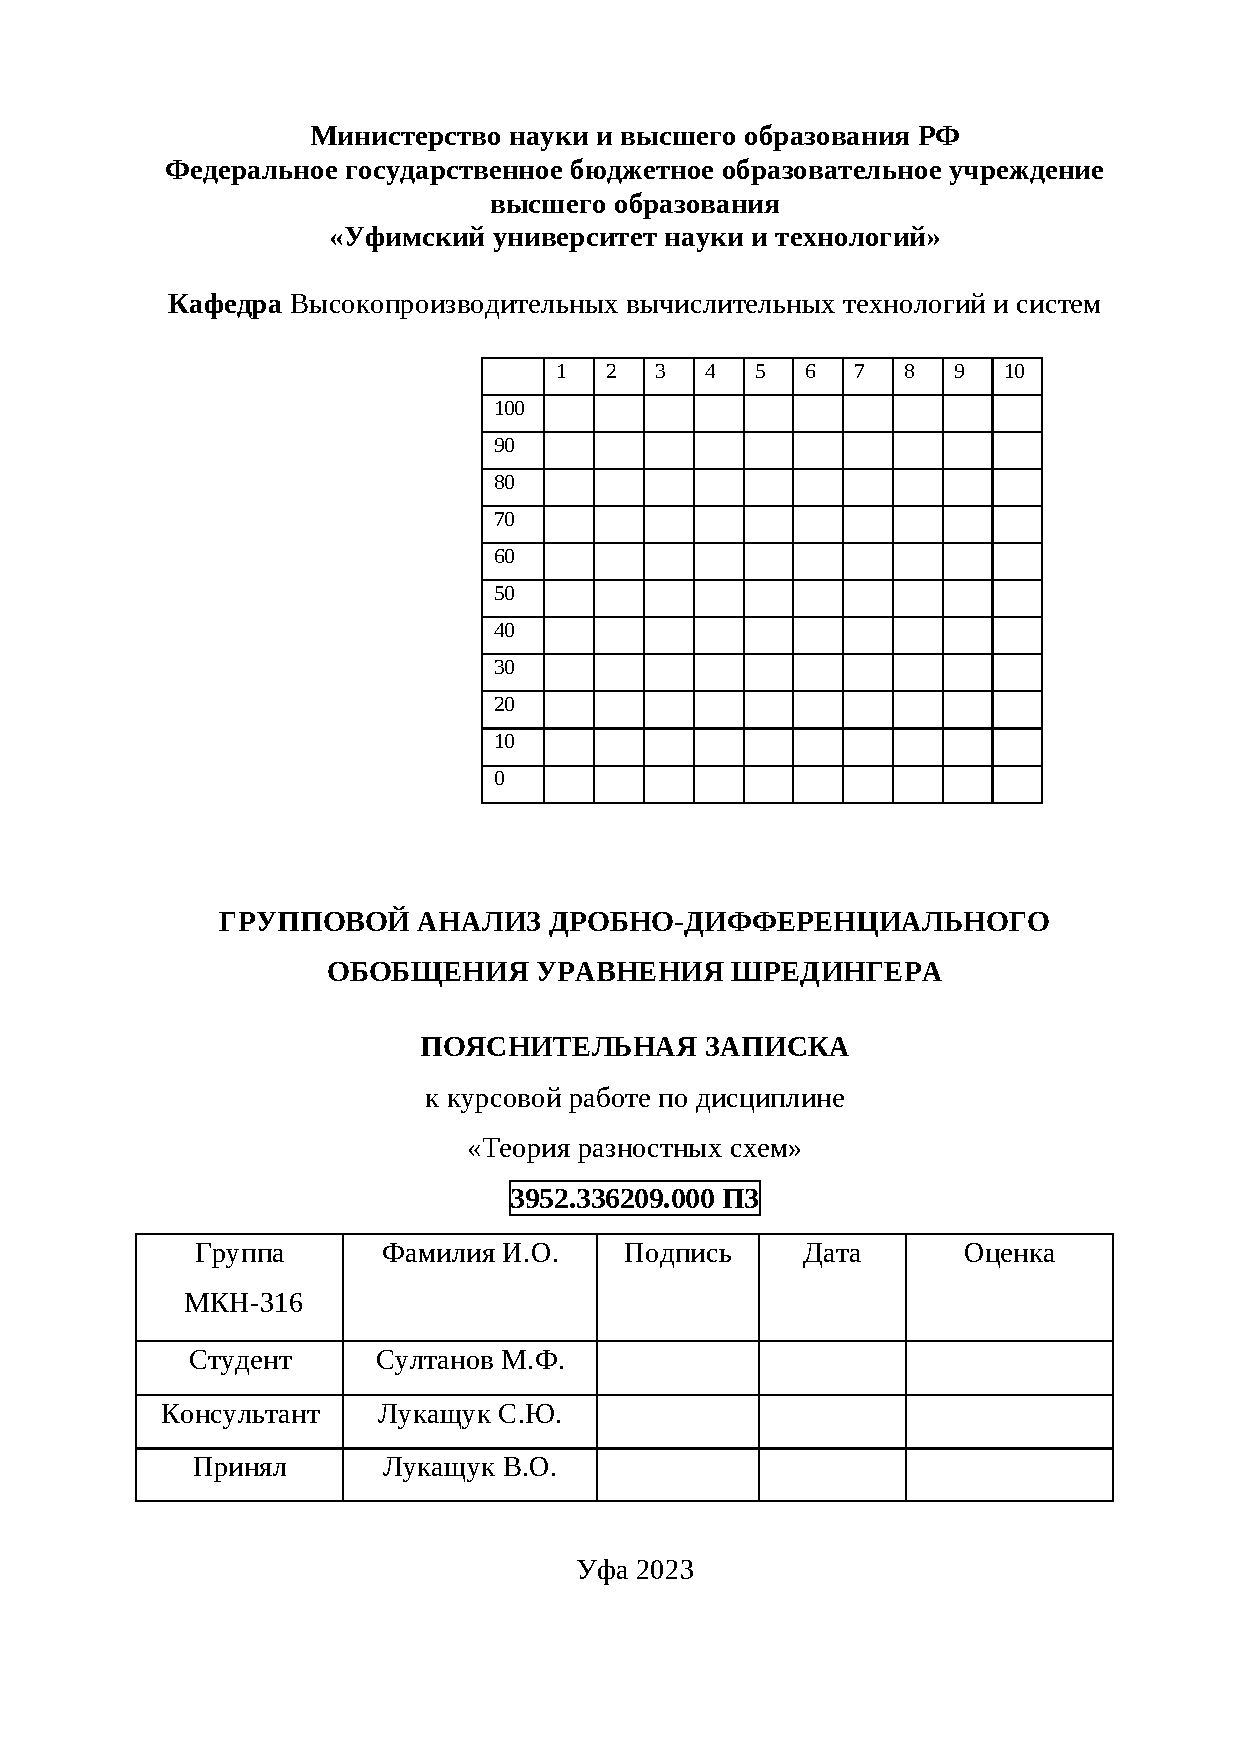
\includepdf[pages={1-3}]{extra.pdf}
% \includepdf[pages={1-3}]{src/word pdfs.pdf} % титульник
\tableofcontents

\newpage
\section*{ВВЕДЕНИЕ}
\addcontentsline{toc}{section}{Введение}


Целью данной работы является исследование свойств симметрии дробно-дифференциального обобщения уравнения Шредингера, полученное путем замены обычных производных на дробные производные Римана-Лиувилля и Маршо.

Для достижения данной цели необходимо выполнить задачи:

\begin{itemize}
  \item Методами группового анализа в случае оператора Римана-Лиувилля
  \begin{itemize}
    \item вывести формулы координат продолжения инфинитиземального генератора группы
    \item решить определяющую систему и найти координаты допускаемых операторов
  \end{itemize}
  \item В случае производных Маршо проверить наличие симметрий, полученных на предыдущем шаге, а также исследовать уравнение на наличие симметрии Галиллея.
\end{itemize}


\newpage
\section[Теоретическая часть]{ТЕОРЕТИЧЕСКАЯ ЧАСТЬ}

\subsection[Основные сведения о дробных производных Римана-Лиувилля и Маршо]{ОСНОВНЫЕ СВЕДЕНИЯ О ДРОБНЫХ ПРОИЗВОДНЫХ РИМАНА-ЛИУВИЛЛЯ И МАРШО}

Фундаментальное введение в теорию дробных прозводных можно найти в монографии \cite{samko}.
В данной работе кратко приведем основные сведения о дробных производных  Римана-Лиувилля и Маршо, необходимые
для группового анализа дробно-дифференциальных уравнений.

Большинство доказательств приведенных ниже формул можно найти, например, в \cite{kasatkin-disert} и \cite{luka}.

Рассмотрим функцию $f(x) \in L_1(a, b)$, где $(a, b)$ конечный интервал.


\textbf{Определение.} Интегро-дифференциальное выражение
\begin{equation}
  \label{eq:RLD_left}
  \RLD{a}{x}{f}(x) = \frac{1}{\Gamma(n-\alpha)} \frac{d^n}{dx^n} \int_{a}^{x} \frac{f(\xi)}{(x-\xi)^{\alpha-n+1}} d \xi
\end{equation}
где $\alpha > 0, n = [\alpha] + 1$ называется левосторонней дробной производной Римана-Лиувилля порядка $\alpha$.


\textbf{Определение.}  Интегро-дифференциальное выражение
\begin{equation}
  \label{eq:RLD_right}
  \RLD{x}{b}{f}(x) = \frac{(-1)^n}{\Gamma(n-\alpha)} \frac{d^n}{dx^n} \int_{x}^{b} \frac{f(\xi)}{(\xi-x)^{\alpha-n+1}} d \xi
\end{equation}
где $\alpha > 0, n = [\alpha] + 1$ называется правосторонней дробной производной Римана-Лиувилля порядка $\alpha$.



\textbf{Утверждение.}  При переходе к пределу $\alpha \rightarrow n, n \in \mathbb{N}$, дробные производные \eqref{eq:RLD_left} и \eqref{eq:RLD_right} переходят в производную целого порядка $f^{(n)}(x)$.


\textbf{Утверждение.} Если $f(x), g(x)$ аналитические функции, то справедливо обобщенное правило Лейбница:
\begin{equation}
  \RLD{x}{b}{f(x) g(x)} = \sum_{n = 0}^{\infty} \binom{\alpha}{n} (-1)^n \RLDa{x}{b}{f(x)}{\alpha-n} \D{x}{n}{g(x)}
\end{equation}

\begin{equation}
  \RLD{a}{x}{f(x) g(x)} = \sum_{n = 0}^{\infty} \binom{\alpha}{n} \RLDa{a}{x}{f(x)}{\alpha-n} \D{x}{n}{g(x)}
\end{equation}
где биномиальные коэффициенты определяются через гамма-функцию:
\begin{equation*}
  \binom{p}{q} = \frac{\Gamma(p+1)}{\Gamma(q+1) \Gamma(p-q+1)}
\end{equation*}

\textbf{Утверждение.}  Пусть $f(x) \in AC^n [a, b]$, тогда справедливы равенства:

\begin{equation}
  \RLD{x}{b}{g(x) f'(x)} = (-1)^n \left( \RLDa{x}{b}{g(x) f(x)}{\alpha + 1} \right) - \RLD{x}{b}{f(x) \D{x}{}{g(x)}}
\end{equation}

\begin{equation}
  \RLD{a}{x}{g(x) f'(x)} = \RLDa{a}{x}{g(x) f(x)}{\alpha + 1} - \RLD{a}{x}{f(x) \D{x}{}{g(x)}}
\end{equation}

Теперь рассмотрим случай бесконечного интервала. Следуя \cite{samko}, введем операторы дробной производной Маршо.
Они оказывается очень удобными при обобщении операторов \eqref{eq:RLD_left} и \eqref{eq:RLD_right} на случай $x\in (-\infty, \infty)$.
В той же монографии приведены условия, предъявляемые для функции, для которой будет определено применение оператора (см. теорему 5.9).
Следует отметить то, что производные Маршо и Римана-Лиувилля в случае бесконечного интервала совпадают на достаточно широком классе функций.

\textbf{Определение.} Лево- и правосторонней дробной производной Маршо порядка $\alpha > 1$ будем называть операторы:
\begin{equation}
  \MD{+}{f(x)} = \frac{\{ \alpha \}}{\Gamma(1 - \{\alpha\})} \int_0^\infty\frac{f^{(n)}(x) - f^{(n)}(x-\xi)}{\xi^{1 + \{\alpha\}}} d\xi
\end{equation}
\begin{equation}
  \label{eq:MD_xux}
  \MD{-}{f(x)} = \frac{\{ \alpha \}}{\Gamma(1 - \{\alpha\})} \int_0^\infty\frac{f^{(n)}(x) - f^{(n)}(x+\xi)}{\xi^{1 + \{\alpha\}}} d\xi
\end{equation}

Здесь $n = [\alpha], \alpha = n + \{\alpha\}$.


\textbf{Утверждение.} Производные маршо от константы равны нулю.

Для дальнейших вычислений нам потребуется ормула:
\begin{equation}
  \MD{\pm}{x f'(x)} = \MD{\pm}{f(x)}  + x \MD{\pm}{f'(x)} 
\end{equation}

% Производные маршо определены на функциях $f(x) \in C^{[\alpha]}(\mathbb{R})$ таких, что 
% \begin{equation*}
%   \sup_{x \in \mathbb{R}} |f(x)| < \infty \text{и} |f^{([\alpha])}(x+h)-f^{([\alpha])}(x)| \leq A(x) h^\lambda, \quad \lambda > \alpha - [\alpha]
% \end{equation*}

\subsection[Алгоритм поиска симметрий дробно-дифференциальных уравнений]{АЛГОРИТМ ПОИСКА СИММЕТРИЙ ДРОБНО-ДИФФЕРЕНЦИАЛЬНЫХ УРАВНЕНИЙ}

Подробно теория классического группового анализа изложена в \cite{ibragimov}.
Анализ в случае функции одной переменной с оператором дробной производной Римана-Лиувилля подробно рассмотрен в \cite{luka} и \cite{kasatkin-disert}.


Алгоритм построения допускаемых генераторов группы симметрий дифференциального уравнения $F = F(t, x, u, \dots,\varDelta_{i}, \dots)$, где $\varDelta_{i}$ - некоторый оператор.

\begin{enumerate}
  \item Рассматриваются инфинитезимальные операторы $X$ вида:
  \begin{equation*}
    X = \xi^t(t, x, u) \frac{\partial}{\partial t}  + \xi^x(t, x, u)  \frac{\partial}{\partial x}  + \eta^u(t, x, u)  \frac{\partial}{\partial u}
  \end{equation*}
  \item Формула продолжения в общем виде:
  \begin{equation}
    \label{eq:cont}
    \begin{split}
      {\huge \zeta}_{Lu} = L\left(\eta^u - \sum_{i=0}^{n} \xi^i u_i \right) + \sum_{i=0}^{n} \xi^i \D{i}{}{L u}
    \end{split}
  \end{equation}
  \item Координаты допускаемых операторов ищутся из определяющего уравнения:
  \begin{equation*}
    (\tilde{X}F)\bigg|_{F=0} = 0
  \end{equation*}
  здесь $\tilde{X}$ - продолженный на необходимые производные оператор $X$.
\end{enumerate}

В случае ДУЧП дробного порядка вида: $$ F(t, x, u, u_t, \RLD{a}{x}{u}, \RLD{x}{b}{u})$$ алгоритм требует некоторых изменений.

\begin{enumerate}
  \item Рассматриваются инфинитезимальные операторы $X$ вида:
  \begin{equation*}
    X = \xi^t(t, x, u) \frac{\partial}{\partial t}  + \xi^x(t, x, u)  \frac{\partial}{\partial x}  + \eta^u(t, x, u)  \frac{\partial}{\partial u}
  \end{equation*}
  где $\xi^t$ и $\xi^x$ такие, что допускается симметрия $x-a = 0$ и $x-b = 0$
  (условие инвариантности оператора относительно замены переменных).

  \item Формулы продолжений запишутся в виде:
\begin{equation}
  \label{eq:cont_t}
  \zeta_{\frac{\partial u}{\partial t}} = \D{t}{}{\eta^u} - u_t \D{t}{}{\xi^t}- u_x \D{t}{}{\xi^x}
\end{equation}
\begin{equation}
  \label{eq:cont_RL_left}
  \begin{split}\zeta_{\RLD{a}{x}{u}} = \RLD{a}{x}{\eta^u} &+ \sum_{n=0}^{\infty} \binom{\alpha}{n} \frac{n-\alpha}{n+1} \RLDa{a}{x}{u}{\alpha - n} \D{x}{n+1}{\xi^x} - \\
    &- \sum_{n=1}^{\infty} \binom{\alpha}{n} \RLDa{a}{x}{u_t}{\alpha-n} \D{x}{n}{\xi^t}
  \end{split}
\end{equation}
\begin{equation}
  \label{eq:cont_RL_right}
  \begin{split}\zeta_{\RLD{x}{b}{u}} = \RLD{x}{b}{\eta^u} &+ \sum_{n=0}^{\infty} \binom{\alpha}{n} (-1)^n \frac{n-\alpha}{n+1} \RLDa{x}{b}{u}{\alpha - n} \D{x}{n+1}{\xi^x} - \\
    &- \sum_{n=1}^{\infty} \binom{\alpha}{n} (-1)^n \RLDa{x}{b}{u_t}{\alpha-n} \D{x}{n}{\xi^t}
  \end{split}
\end{equation}

Однако, расчет можно сильно упростить. Положим, что
\begin{equation}
  \label{eq:linear_autonom}
  \xi^x = \xi^x(t, x), \quad \xi^t = \xi^t(t, x), \quad \eta^u = \eta_0^u(t, x) + \eta^u_1 u.
\end{equation}

Такие однопараметрические группы преобразований с координатами \eqref{eq:linear_autonom} называются группами линейно-автономных преобразований.

Дробно-дифференциальные операторы не обладают свойством линеаризации. Это связано с их нелокальностью в отличие от операторов целочисленного дифференцирования. Поэтому нелинейные преобразования не могут преобразовывать линейный дробный оператор в оператор того же вида. На данный момент неизвестно ни одной симметрии дробно-дифференциальных уравнений, не являющейся линейно-автономной симметрией (подробнее см. \cite{luka} стр. 138).

В таких предоположениях координаты можно вычислить по формулам:
\begin{equation}
  \label{eq:cont_RL_left_la}
  \begin{split}\zeta_{\RLD{a}{x}{u}} = \RLD{a}{x}{\eta^u_0} &+ \sum_{n=0}^{\infty} \binom{\alpha}{n} \RLDa{a}{x}{u}{\alpha - n}  \left( \D{x}{n}{\eta^u_1} + \frac{n-\alpha}{n+1} \D{x}{n+1}{\xi^x} \right)- \\
    &- \sum_{n=1}^{\infty} \binom{\alpha}{n} \RLDa{a}{x}{u_t}{\alpha-n} \D{x}{n}{\xi^t}
  \end{split}
\end{equation}
\begin{equation}
  \label{eq:cont_RL_right_la}
  \begin{split}\zeta_{\RLD{x}{b}{u}} = \RLD{x}{b}{\eta^u_0} &+ \sum_{n=0}^{\infty} \binom{\alpha}{n} \RLDa{x}{b}{u}{\alpha - n} \left( \D{x}{n}{\eta^u_1} + (-1)^n \frac{n-\alpha}{n+1}  \D{x}{n+1}{\xi^x} \right)- \\
    &- \sum_{n=1}^{\infty} \binom{\alpha}{n} (-1)^n \RLDa{x}{b}{u_t}{\alpha-n} \D{x}{n}{\xi^t}
  \end{split}
\end{equation}
  \item Координаты допускаемых операторов ищутся из определяющего уравнения:
  \begin{equation*}
    (\tilde{X}F)\bigg|_{F=0} = 0
  \end{equation*}
  $$\tilde{X} = X + \zeta^0 \frac{\partial}{\partial u_t} + \zeta^1 \frac{\partial}{\partial \RLD{a}{x}{u}}+ \zeta^2 \frac{\partial}{\partial \RLD{x}{b}{u}}$$ $\zeta^0, \zeta^1, \zeta^2$ определяются соответственно по формулам \eqref{eq:cont_t}, \eqref{eq:cont_RL_left_la}, \eqref{eq:cont_RL_right_la}.
\end{enumerate}

Данный алгоритм можно обобщить и на случай системы ДУЧП дробного порядка.
\section[Практическая часть]{ПРАКТИЧЕСКАЯ ЧАСТЬ}
\subsection[Поиск симметрий дробно-дифференциального обобщения уравнения Шредингера с производными Римана-Лиувилля]{ПОИСК СИММЕТРИЙ ДРОБНО-ДИФФЕРЕНЦИАЛЬНОГО ОБОБЩЕНИЯ УРАВНЕНИЯ ШРЕДИНГЕРА С ПРОИЗВОДНЫМИ РИМАНА-ЛИУВИЛЛЯ}

Рассматривается дробно-дифферециальное обобщение уравнение Шредингера:
\begin{equation}
  \label{eq:shredinger_RL_inline}
  i \cfrac{\partial \psi}{\partial t} = \RLD{a}{x}{\psi} + \RLD{x}{b}{\psi}, \quad \alpha \in (1, 2), \quad t > 0, \quad x \in [a, b]
\end{equation}

Представим функцию $\psi(t, x)$ в виде:

\begin{equation*}
  \psi(t, x) = u(t, x) + i v(t, x)
\end{equation*}

Тогда \eqref{eq:shredinger_RL_inline} можно записать в виде системы:

\begin{equation}
  \label{eq:shredinger_RL_system}
  \begin{cases}
    \cfrac{\partial u}{\partial t} = \RLD{a}{x}{v} + \RLD{x}{b}{v} \\
    \cfrac{\partial v}{\partial t} = - \left( \RLD{a}{x}{u} + \RLD{x}{b}{u} \right)
  \end{cases}
\end{equation}


Инфинитезимальный генератор будем искать в виде:
\begin{equation*}
  X = \tau \frac{\partial}{\partial t}  + \xi \frac{\partial}{\partial x}  + \mu \frac{\partial}{\partial u}  + \vartheta  \frac{\partial}{\partial v}
\end{equation*}

Тогда инфинитезимальный оператор продолженной группы имеет вид:
\begin{equation}
  \label{eq:generator}
  \begin{split}
    \tilde{X} = X &+ \left(\zeta^u \frac{\partial }{\partial u_t} + \rho^u \frac{\partial }{\partial (\RLD{a}{x}{u})} + \lambda^u \frac{\partial }{\partial (\RLD{x}{b}{u})} \right) +\\
    &+\left(\zeta^v \frac{\partial }{\partial v_t}  + \rho^v \frac{\partial }{\partial (\RLD{a}{x}{v})}  + \lambda^v \frac{\partial }{\partial (\RLD{x}{b}{v})} \right)
  \end{split}
\end{equation}

Координаты $\zeta^u, \zeta^v$ будут иметь вид \eqref{eq:cont_t}, $\rho^u, \rho^v$ вид \eqref{eq:cont_RL_left_la}, а $\lambda^u, \lambda^v$ соответственно вид \eqref{eq:cont_RL_right_la}.

Применим генератор \eqref{eq:generator} к системе \eqref{eq:shredinger_RL_system}:

\begin{equation}
  \begin{cases}
    \zeta^u = \rho^v + \lambda^v \\
    \zeta^v = - (\rho^u + \lambda^u)
  \end{cases}
\end{equation}

Определяющая система примет следующий вид:
\begin{equation}
  \label{eq:RL_def_sys}
  \begin{cases}
    \begin{aligned}
      u \D{t}{}{\mu_1} + \D{t}{}{\mu_0} + \left(\RLD{a}{x}{v} + \RLD{x}{b}{v}\right) \left(\mu_1 + \D{t}{}{\tau} \right) -  \D{x}{}{u} \D{t}{}{\xi} =                                     \\
      = \RLD{a}{x}{\vartheta _0} + \sum_{n=0}^{\infty} \binom{\alpha}{n} \RLDa{a}{x}{v}{\alpha - n}  \left( \D{x}{n}{\vartheta _1} + \frac{n-\alpha}{n+1} \D{x}{n+1}{\xi} \right)+        \\
      + \RLD{x}{b}{\vartheta _0} + \sum_{n=0}^{\infty} \binom{\alpha}{n} \RLDa{x}{b}{v}{\alpha - n} \left( \D{x}{n}{\vartheta _1} + (-1)^n \frac{n-\alpha}{n+1}  \D{x}{n+1}{\xi} \right)+ \\
      + \sum_{n=1}^{\infty} \binom{\alpha}{n} \RLDa{a}{x}{\RLD{a}{x}{u} + \RLD{x}{b}{u}}{\alpha-n} \D{x}{n}{\tau} +                                                                       \\
      + \sum_{n=1}^{\infty} \binom{\alpha}{n} (-1)^n \RLDa{x}{b}{\RLD{a}{x}{u} + \RLD{x}{b}{u}}{\alpha-n} \D{x}{n}{\tau}
    \end{aligned} \\

    \begin{aligned}
      v \D{t}{}{\vartheta _1} + \D{t}{}{\vartheta _0} + \left(\RLD{a}{x}{u} + \RLD{x}{b}{u}\right) \left(\D{t}{}{\tau} - \vartheta _1 \right) -  \D{x}{}{v} \D{t}{}{\xi} =  \\
      = - \RLD{a}{x}{\mu_0} - \sum_{n=0}^{\infty} \binom{\alpha}{n} \RLDa{a}{x}{u}{\alpha - n}  \left( \D{x}{n}{\mu_1} + \frac{n-\alpha}{n+1} \D{x}{n+1}{\xi} \right)-      \\
      - \RLD{x}{b}{\mu_0} + \sum_{n=0}^{\infty} \binom{\alpha}{n} \RLDa{x}{b}{u}{\alpha - n} \left( \D{x}{n}{\mu_1} + (-1)^n \frac{n-\alpha}{n+1}  \D{x}{n+1}{\xi} \right)+ \\
      + \sum_{n=1}^{\infty} \binom{\alpha}{n} \RLDa{a}{x}{\RLD{a}{x}{v} + \RLD{x}{b}{v}}{\alpha-n} \D{x}{n}{\tau} +                                                         \\
      + \sum_{n=1}^{\infty} \binom{\alpha}{n} (-1)^n \RLDa{x}{b}{\RLD{a}{x}{v} + \RLD{x}{b}{v}}{\alpha-n} \D{x}{n}{\tau}
    \end{aligned}
  \end{cases}
\end{equation}

Расщепив систему \eqref{eq:RL_def_sys} по $u$ и $v$ (первые слагаемые в каждой системе), можно сделать вывод о том, что $\mu_1 = \mu_1(x), \vartheta _1 = \vartheta _1(x)$.

Если расщепить по $\RLDa{a}{x}{v}{\alpha - n}$, то получим, что
\begin{equation}
  \label{eq:UwU}
  \D{x}{n}{\vartheta _1} + \frac{n - \alpha}{n + 1} \D{x}{n+1}{\xi}  = 0
\end{equation}

Рассмотрим слагаемые \eqref{eq:UwU} при $n = 1$ и $n = 2$:
\begin{gather}
  \label{eq:UwUwU_1}\D{x}{1}{\vartheta _1} + \frac{1 - \alpha}{2} \D{x}{2}{\xi} = 0 \\
  \label{eq:UwUwU_2}\D{x}{2}{\vartheta _1} + \frac{2 - \alpha}{3} \D{x}{3}{\xi} = 0
\end{gather}

Продифференцируем \eqref{eq:UwUwU_1} по x и из полученного выражения вычтем \eqref{eq:UwUwU_2}, получим, что:

\begin{equation}
  \label{eq:xi}
  \D{x}{3}{\xi} = 0 \Rightarrow \xi = A x^2 + B x + C
\end{equation}

Подставляя \eqref{eq:xi} в \eqref{eq:UwUwU_2} получаем, что:
\begin{equation}
  \label{eq:nu_1}
  \D{x}{2}{\vartheta _1} = 0 \Rightarrow \vartheta _1 = D x + E
\end{equation}

Теперь расщепим по $\RLDa{x}{b}{v}{\alpha - n}$ при $n > 0$, аналогично получаем:
\begin{gather}
  \label{eq:Meow_1}\D{x}{1}{\vartheta _1} - \frac{1 - \alpha}{2} \D{x}{2}{\xi} = 0 \\
  \label{eq:Meow_2}\D{x}{2}{\vartheta _1} + \frac{2 - \alpha}{3} \D{x}{3}{\xi} = 0
\end{gather}

Подставим \eqref{eq:nu_1} в \eqref{eq:Meow_1}, тогда:
\begin{equation}
  \label{eq:AAA}
  D = (1 - \alpha) A
\end{equation}

Но, из \eqref{eq:UwUwU_1}:

\begin{equation}
  \label{eq:BBB}
  D + (1 - \alpha) A = 0 \Rightarrow D = - (1 - \alpha) A
\end{equation}

Значит, из \eqref{eq:AAA} и \eqref{eq:BBB} следует:
\begin{equation*}
  D = A = 0
\end{equation*}

Расщепим по $\RLDa{x}{b}{u}{\alpha - n}$ при $n > 0$ (аналогично можно расмотреть $\RLDa{a}{x}{u}{\alpha - n}$), получим:
\begin{gather*}
  \label{eq:Gav_1}\D{x}{1}{\mu_1} - \frac{1 - \alpha}{2} \D{x}{2}{\xi} = 0 \\
  \label{eq:Gav_2}\D{x}{2}{\mu_1} + \frac{2 - \alpha}{3} \D{x}{3}{\xi} = 0
\end{gather*}

Cравнивая с \eqref{eq:Meow_1} и \eqref{eq:Meow_2}, заключаем:
\begin{equation*}
  \mu_1 = \vartheta _1 = E
\end{equation*}

Теперь расщепим по $\RLD{a}{x}{v}$ и $\RLD{a}{x}{u}$, получим равенства:
\begin{gather}
  \mu_1 - \D{t}{}{\tau} = \vartheta _1 - \alpha \D{x}{}{\xi} \\
  -\vartheta _1 + \D{t}{}{\tau} = - \mu_1 + \alpha \D{x}{}{\xi}
\end{gather}

Откуда получаем, что:
\begin{equation}
  \begin{aligned}
    \D{t}{}{\tau} = \alpha \D{x}{}{\xi} = \alpha B \\
    \tau = \alpha B t + f(x)
  \end{aligned}
\end{equation}

Расщепим теперь слагаемые вида:
\begin{equation*}
  \sum_{n=1}^{\infty} \binom{\alpha}{n} \RLDa{a}{x}{\RLD{a}{x}{v} + \RLD{x}{b}{v}}{\alpha-n} \D{x}{n}{\tau}
\end{equation*}

Тогда можно заключить, что:
\begin{equation*}
  \D{x}{n}{\tau} = 0 \rightarrow \D{x}{1}{\tau}s = f'(x) = 0 \rightarrow f(x) = F \equiv const
\end{equation*}

\begin{equation}
  \tau = \alpha B t + F
\end{equation}

Из оставшихся слагаемых получаем систему:
\begin{equation}
  \label{eq:infinity_group}
  \begin{cases}
    \D{t}{}{\mu_0} = \RLD{a}{x}{\vartheta_0} + \RLD{x}{b}{\vartheta_0} \\
    \D{t}{}{\vartheta_0} = - \RLD{a}{x}{\mu_0} - \RLD{x}{b}{\mu_0}
  \end{cases}
\end{equation}

Таким образом, функции $\mu_0$ и $\vartheta_0$ остаются произвольными функциями, удовлетворяющие системе \eqref{eq:infinity_group},
пораждая бесконечномерную группу преобразований. %TODO каких преобразований??%

Следующие группы переносов:
\begin{equation*}
  X = \frac{\partial}{\partial x} \quad X = \frac{\partial}{\partial t}
\end{equation*}

Не допускаются системой \eqref{eq:shredinger_RL_system}, поскольку не удовлетворяют условию:

\begin{equation*}
  \xi |_{x = 0} = 0 \quad \text{и} \quad \tau|_{t = 0} = 0
\end{equation*}

Таким образом, получаем следующие инфинитезимальные генераторы:

\begin{equation}
  \label{eq:semi_rotation}
  X_1 = (u + \mu_0(t, x))\frac{\partial}{\partial u} + (v + \vartheta_0(t, x))\frac{\partial}{\partial v}
\end{equation}
\begin{equation}
  X_2 = t \frac{\partial}{\partial t} + x \frac{\partial}{\partial x}
\end{equation}

% Частным случаем \eqref{eq:semi_rotation} при $\mu_0 = v - u$ и $\vartheta_0 = -u - v$ будет преобразование вращения:
% \begin{equation*}
%   X = v \frac{\partial}{\partial u} - u \frac{\partial}{\partial v}
% \end{equation*}

\subsection[Поиск симметрий дробно-дифференциального обобщения уравнения Шредингера с производными Маршо]{ПОИСК СИММЕТРИЙ ДРОБНО-ДИФФЕРЕНЦИАЛЬНОГО ОБОБЩЕНИЯ УРАВНЕНИЯ ШРЕДИНГЕРА С ПРОИЗВОДНЫМИ МАРШО}

Теперь рассмотрим дробно-дифференциальное обобщение уравнения Шредингера на всей числовой оси.
Как уже было показано (см. теоретическую часть), для этого удобно переходить к производным Маршо.
Уравнение принимает вид:

\begin{equation}
  \label{eq:shredinger_MD_inline}
  i \cfrac{\partial \psi}{\partial t} = \MD{+}{\psi} + \MD{-}{\psi}, \quad \alpha \in (1, 2), \quad t > 0, \quad x \in (-\infty, \infty)
\end{equation}

Аналогично предыдущему пункту полагаем $\psi(t, x) = u(t, x) + i v(t, x)$ и приходим к системе:

\begin{equation}
  \label{eq:shredinger_MD_system}
  \begin{cases}
    \cfrac{\partial u}{\partial t} = \quad \MD{+}{v} + \MD{-}{v} \\
    \cfrac{\partial v}{\partial t} = - \left( \MD{+}{u} + \MD{-}{u} \right)
  \end{cases}
\end{equation}

Общего алгоритма поиска симметрий для оператора дробной производной Маршо нет.
Поэтому ограничимся лишь проверкой некоторых симметрий.

Инфинитезимальный генератор будем искать в виде:
\begin{equation*}
  X = \tau \frac{\partial}{\partial t}  + \xi \frac{\partial}{\partial x}  + \mu \frac{\partial}{\partial u}  + \vartheta  \frac{\partial}{\partial v}
\end{equation*}

Тогда инфинитезимальный оператор продолженной группы имеет вид:
\begin{equation}
  \label{eq:generator_md}
  \begin{split}
    \tilde{X} = X &+ \left(\zeta^u \frac{\partial }{\partial u_t} + \rho^u \frac{\partial }{\partial (\MD{+}{u})} + \lambda^u \frac{\partial }{\partial (\MD{-}{u})} \right) +\\
    &+\left(\zeta^v \frac{\partial }{\partial v_t}  + \rho^v \frac{\partial }{\partial (\MD{+}{v})}  + \lambda^v \frac{\partial }{\partial (\MD{-}{v})} \right)
  \end{split}
\end{equation}

Координаты $\zeta^u, \zeta^v$ будут определяться по формуле \eqref{eq:cont_t}, остальные координаты представим в общем виде \eqref{eq:cont}:

Применим оператор \eqref{eq:generator_md} к системе \eqref{eq:shredinger_MD_system}:
\begin{equation}
  \label{eq:def_md}
  \begin{cases}
    \begin{aligned}
      \D{t}{}{\mu} & - u_t \D{t}{}{\tau} - u_x \D{t}{}{\xi}  =                                                     \\
      =            & \MD{-}{\vartheta  - \xi v_x - \tau v_t } + \xi \D{x}{}{\MD{-}{v}} + \tau \D{t}{}{\MD{-}{v}} + \\
      +            & \MD{+}{\vartheta  - \xi v_x - \tau v_t } + \xi \D{x}{}{\MD{+}{v}} + \tau \D{t}{}{\MD{+}{v}}
    \end{aligned} \\
    \begin{aligned}
      \D{t}{}{\vartheta } & - v_t \D{t}{}{\tau} - v_x \D{t}{}{\xi}  =                                              \\
      =                   & - \left(\MD{-}{\mu - \xi u_x - \tau u_t } + \xi \D{x}{}{\MD{-}{u}} + \tau \D{t}{}{\MD{-}{u}} \right)+ \\
      +                   & - \left(\MD{+}{\mu  - \xi u_x - \tau u_t } + \xi \D{x}{}{\MD{+}{u}} + \tau \D{t}{}{\MD{+}{u}}\right)
    \end{aligned}
  \end{cases}
\end{equation}

Это не определяющая система, но для удобства будем в неё подставлять различные симметрии, а затем, если это будет необходимо, будем делать замену в силу исходной системы \eqref{eq:shredinger_MD_system}.
\begin{enumerate}
  \item $\xi = 1, \tau = 0, \mu = 0, \vartheta = 0$. Поскольку производная Маршо от константы равна нулю, то данные координаты в явном виде обнуляют систему \eqref{eq:def_md}.
  \item $\xi = 0, \tau = 1, \mu = 0, \vartheta = 0$. Аналогично предыдущему пункту.
  \item $\xi = x, \tau = t, \mu = 0, \vartheta = 0$.
        \begin{equation*}
          \begin{aligned}
            -u_t = & \MD{-}{-x v_x - t v_t} + x \D{x}{}{\MD{-}{v}} + t \D{t}{}{\MD{-}{v}} + \\
            +      & \MD{+}{-x v_x - t v_t} + x \D{x}{}{\MD{+}{v}} + t \D{t}{}{\MD{+}{v}}
          \end{aligned}
        \end{equation*}

        В условиях существования производных Маршо от функций $u, v$  можно поменять порядок интегрирования и дифференцирования. Тогда некоторые слагаемые сократятся:
        \begin{equation*}
          \begin{aligned}
            -u_t = & \MD{-}{-x v_x} + x \MD{-}{v_x} + \MD{+}{-x v_x} + x \MD{+}{v_x}
          \end{aligned}
        \end{equation*}

        Используя формулу \eqref{eq:MD_xux}:
        \begin{equation*}
          \begin{aligned}
            -u_t = & - \MD{-}{v} - x \MD{-}{v_x} + x \MD{-}{v_x} - \MD{+}{v} - x \MD{+}{v_x} + x \MD{+}{v_x}
          \end{aligned}
        \end{equation*}
        \begin{equation*}
          \begin{aligned}
            u_t = & \MD{-}{v} \MD{+}{v}
          \end{aligned}
        \end{equation*}

        В силу \eqref{eq:shredinger_MD_system} получаем тождественное равенство.
        Аналогичное тождество получаем у второго уравнения системы \eqref{eq:def_md}.

  \item $\xi = 0, \tau = 0, \mu = u, \vartheta = v$. После постановки в явном виде получаем систему \eqref{eq:def_md}.
  \item $\xi = 0, \tau = 0, \mu = -v, \vartheta = u$. Аналогично получаем систему \eqref{eq:def_md}.
\end{enumerate}

Таким образом, все основные симметрии, допускаемые уравнением \eqref{eq:shredinger_RL_inline} на конечном отрезке допускаются и в случае бесконечного интервала.

Заметим, однако, что в предельном случае $\alpha = 2$, то есть когда дробные производные переходят в классическую вторую производную,уравнение будет допускать аналог преобразования Галлилея при:
\begin{equation*}
  \xi = t, \tau = 0, \mu = \frac{1}{4} xv, \vartheta = - \frac{1}{4} xu
\end{equation*}

Попробуем проверить будет ли иметь место аналог такого преобразования в случае дробного порядка на бесконечном интервале. Положим:
\begin{equation*}
  \xi = t, \tau = 0
\end{equation*}

Подставим их в \eqref{eq:def_md}, получим:
\begin{equation*}
  \begin{cases}
    \mu_t - u_x = \MD{+}{\vartheta} + \MD{-}{\vartheta} \\
    \vartheta_t - v_x = -\MD{+}{\mu} - \MD{-}{\mu}
  \end{cases}
\end{equation*}

По аналогии с предельным случаем $\alpha = 2$  положим $\mu = \beta x v, \vartheta = - \beta x u$. Тогда для первого уравнения системы:
\begin{equation*}
  u_x = \beta \left(\mathbb{D}_{+}^{\alpha-1}[u] + \mathbb{D}_{-}^{\alpha-1}[u]\right)
\end{equation*}

Данное равенство возможно только в случае целого $\alpha = 2$.
При любом другом выборе $\mu$ и $\vartheta$ усложняется правая часть уравнения и не удается подобрать такие функции,
чтобы получить необходимую допускаемую симметрию.

Таким образом, найдены следующие симметрии:

\begin{equation*}
  \begin{aligned}
    X_1 =& \frac{\partial}{\partial x}\\
    X_2 =& \frac{\partial}{\partial t}\\
    X_3 =& t \frac{\partial}{\partial t} + x \frac{\partial}{\partial x}\\
    X_4 =& u \frac{\partial}{\partial u} + v \frac{\partial}{\partial v}\\
    X_5 =& -v \frac{\partial}{\partial u} + u \frac{\partial}{\partial v}
  \end{aligned}
\end{equation*}

Отметим, что в отличие от уравнения \eqref{eq:shredinger_RL_inline} с производными Римана-Лиувилля уравнение \eqref{eq:shredinger_MD_inline} с производными Маршо допускает группы переносов вдоль $x$ и $t$.
\newpage
\section*{ЗАКЛЮЧЕНИЕ}
\addcontentsline{toc}{section}{Заключение}
В ходе выполнения курсовой работы был проведен групповой анализ дробно-дифференциального уравнения Шредингера с производными Римана-Лиувилля,
в ходе которого была найдена бесконечномерная алгебра операторов, среди которых есть операторы сдвига и однородного растяжения по времени и пространству.

Все данные операторы также допускаются дробно-дифференциальным уравнением Шредингера с производными Маршо, преобразование Галлилея в том виде, в котором допускается классическим уравнением, найдено не было.
\newpage

\addcontentsline{toc}{section}{Список литературы}
\begin{thebibliography}{9}
  \bibitem{samko}
  Самко С. Г., Килбас А. А., Маричев О. И. Интегралы и производные дробного порядка и некоторые их приложения. Минск: Наука и техника, 1987. 688 с.
  \bibitem{kasatkin-disert}
  Касаткин А. А. Симметрии и точные решения уравнений с производными дробного порядка типа Римана–Лиувилля: Дисс. канд. физ.-мат. наук. 2013. УГАТУ. 118 с.
  \bibitem{luka}
  Лукащук, В. О., С. Ю. Лукащук. Обыкновенные дифференциальные уравнения дробного порядка: основы классической теории и группового анализа. - Уфа: УГАТУ, 2022.
  \bibitem{ibragimov}
  Ибрагимов Н. Х. Группы преобразований в математической физике. М.: Наука, 1983. 280 с.
\end{thebibliography}
\includepdf[pages={4}]{extra.pdf}
% \includepdf[pages={17-31}]{src/word pdfs.pdf}
\end{document}


